\section{取整函数}
\begin{definition}[取整函数]
设\(x\in\mathbb{R},
n\in\mathbb{Z}\),
定义:\begin{enumerate}
	\item 如果\(n\)是不大于\(x\)的最大整数,
	即\(x\in[n,n+1)\),
	那么记\(\floor{x}=n\).
	我们把函数\(y=\floor{x}\)称为\DefineConcept{向下取整函数},
	即\begin{equation}
		\floor{x}
		\defeq
		\max\Set{ n\in\mathbb{Z} \given n \leq x }.
	\end{equation}

	\item 如果\(n\)是不小于\(x\)的最小整数,
	即\(x\in(n-1,n]\),
	那么记\(\ceil{x}=n\).
	我们把函数\(y=\ceil{x}\)称为\DefineConcept{向上取整函数},
	即\begin{equation}
		\ceil{x}
		\defeq
		\min\Set{ n\in\mathbb{Z} \given n \geq x }.
	\end{equation}
\end{enumerate}
\end{definition}

\begin{figure}[htb]
	\tikzstyle{sx}=[draw=orange,fill=orange]
	\tikzstyle{kx}=[draw=orange,fill=white]
	\def\subwidth{.45\linewidth}
	\def\subscale{.9}
	\begin{subfigure}[b]{\subwidth}%
		\centering
		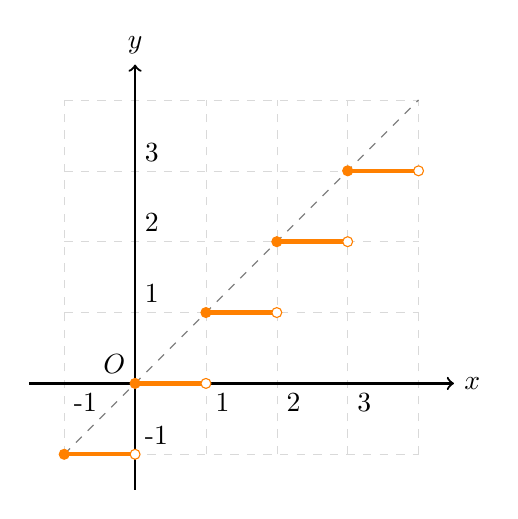
\begin{tikzpicture}[scale=\subscale]
			\draw[help lines, color=gray!30, dashed] (-1,-1) grid (4,4);
			\draw[dashed, color=gray] (-1,-1) -- (4,4);
			\draw[->, thick] (-1.5,0) -- (4.5,0) node[right]{\(x\)};
			\draw[->, thick] (0,-1.5) -- (0,4.5) node[above]{\(y\)};
			\foreach \i in {-1,...,3} {
				\draw[ultra thick,orange] (\i,\i)--(\i+1,\i);
				\fill[sx] (\i,\i)circle(2pt);
				\fill[kx] (\i+1,\i)circle(2pt);
				\ifnum\i=0\relax\else
					\draw(\i,0)node[below right]{\i};
					\draw(0,\i)node[above right]{\i};
				\fi
			}
			\draw (0,0)node[above left]{\(O\)};
		\end{tikzpicture}
		\subcaption{向下取整函数\(\floor{x}\)}
	\end{subfigure}
	\begin{subfigure}[b]{\subwidth}%
		\centering
		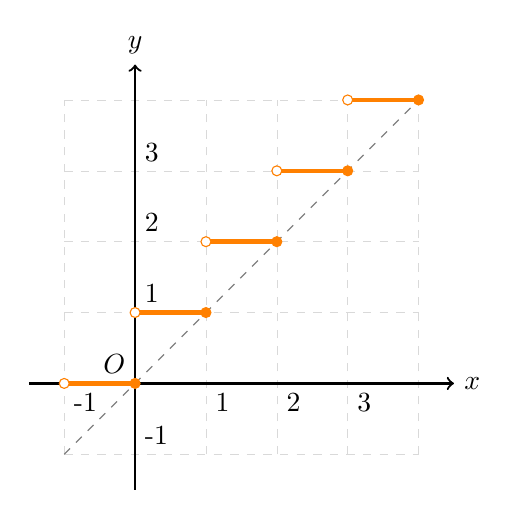
\begin{tikzpicture}[scale=\subscale]
			\draw[help lines, color=gray!30, dashed] (-1,-1) grid (4,4);
			\draw[dashed, color=gray] (-1,-1) -- (4,4);
			\draw[->, thick] (-1.5,0) -- (4.5,0) node[right]{\(x\)};
			\draw[->, thick] (0,-1.5) -- (0,4.5) node[above]{\(y\)};
			\foreach \i in {-1,...,3} {
				\draw[ultra thick,orange] (\i,\i+1)--(\i+1,\i+1);
				\fill[kx] (\i,\i+1)circle(2pt);
				\fill[sx] (\i+1,\i+1)circle(2pt);
				\ifnum\i=0\relax\else
					\draw(\i,0)node[below right]{\i};
					\draw(0,\i)node[above right]{\i};
				\fi
			}
			\draw (0,0)node[above left]{\(O\)};
		\end{tikzpicture}
		\subcaption{向上取整函数\(\ceil{x}\)}
	\end{subfigure}
	\caption{取整函数的图形}
	\label{figure:取整函数.取整函数的图形}
\end{figure}

\begin{figure}
	\tikzstyle{sx}=[draw=orange,fill=orange]
	\tikzstyle{kx}=[draw=orange,fill=white]
	\def\subwidth{.45\linewidth}
	\def\subscale{.9}
	%@Mathematica: Plot[x - Floor[x], {x, -1, 4}]
	%@Mathematica: Table[{x, x - Floor[x]}, {x, -1, 4, .2}] // TableForm
	\begin{subfigure}[b]{\subwidth}%
		\centering
		\begin{tikzpicture}[scale=\subscale]
			\begin{axis}[
				xmin=-1,xmax=4,
				ymin=-1,ymax=1,
				restrict y to domain=-1:1,
				axis lines=middle,
				axis equal=true,
				xlabel=$x$,
				ylabel=$y$,
				enlarge x limits=0.1,
				enlarge y limits=0.1,
				x label style={at={(ticklabel* cs:1.00)}, inner sep=5pt, anchor=south},
				y label style={at={(ticklabel* cs:1.00)}, inner sep=2pt, anchor=west},
				ytick={-1,1},
			]
				\foreach \i in {-1,...,3} {
					\addplot[color=orange,samples=2,domain={\i}:{\i+1}]{x-\i};
				}
				\fill[kx](-1,1)circle(2pt);
				\fill[kx](0,1)circle(2pt);
				\fill[kx](1,1)circle(2pt);
				\fill[kx](2,1)circle(2pt);
				\fill[kx](3,1)circle(2pt);
				\fill[kx](4,1)circle(2pt);
				\fill[sx](-1,0)circle(2pt);
				\fill[sx](0,0)circle(2pt);
				\fill[sx](1,0)circle(2pt);
				\fill[sx](2,0)circle(2pt);
				\fill[sx](3,0)circle(2pt);
				\fill[sx](4,0)circle(2pt);
			\end{axis}
		\end{tikzpicture}
		\subcaption{函数\(f(x)=x-\floor{x}\)}
	\end{subfigure}
	%@Mathematica: Plot[Ceiling[x] - x, {x, -1, 4}]
	%@Mathematica: Table[{x, Ceiling[x] - x}, {x, -1, 4, .2}] // TableForm
	\begin{subfigure}[b]{\subwidth}%
		\centering
		\begin{tikzpicture}[scale=\subscale]
			\begin{axis}[
				xmin=-1,xmax=4,
				ymin=-1,ymax=1,
				axis lines=middle,
				axis equal=true,
				xlabel=$x$,
				ylabel=$y$,
				enlarge x limits=0.1,
				enlarge y limits=0.1,
				x label style={at={(ticklabel* cs:1.00)}, inner sep=5pt, anchor=south},
				y label style={at={(ticklabel* cs:1.00)}, inner sep=2pt, anchor=west},
				ytick={-1,1},
			]
				\foreach \i in {-1,...,3} {
					\addplot[color=orange,samples=2,domain={\i}:{\i+1}]{\i+1-x};
				}
				\fill[kx](-1,1)circle(2pt);
				\fill[kx](0,1)circle(2pt);
				\fill[kx](1,1)circle(2pt);
				\fill[kx](2,1)circle(2pt);
				\fill[kx](3,1)circle(2pt);
				\fill[kx](4,1)circle(2pt);
				\fill[sx](-1,0)circle(2pt);
				\fill[sx](0,0)circle(2pt);
				\fill[sx](1,0)circle(2pt);
				\fill[sx](2,0)circle(2pt);
				\fill[sx](3,0)circle(2pt);
				\fill[sx](4,0)circle(2pt);
			\end{axis}
		\end{tikzpicture}
		\subcaption{函数\(f(x)=\ceil{x}-x\)}
	\end{subfigure}
	\caption{}
\end{figure}

\begin{property}\label{theorem:取整函数.性质1}
%@see: 《算法导论(原书第3版)》 P31 (3.3)
一般地,对于\(x\in\mathbb{R}\),总有\begin{equation}
	x - 1 < \floor{x} \leq x \leq \ceil{x} < x + 1.
\end{equation}
%TODO proof
\end{property}

\begin{example}
设\(x,y\)都是实数.
举例说明:\(\ceil{x} + \ceil{y} \neq \ceil{x+y},
\floor{x} + \floor{y} \neq \floor{x+y}\).
\begin{solution}
%@credit: {6d916ea6-1441-4c5b-9e97-4f834b319710} 说:都取0.5
取\(x = y = \frac12\).
那么\(\ceil{x} = \ceil{y} = \ceil{x+y} = 1\),
但是\(\ceil{x} + \ceil{y} = 2 \neq \ceil{x+y}\).

与此同时,\(\floor{x} = \floor{y} = 0,
\floor{x+y} = 1\),
因此\(\floor{x} + \floor{y} \neq \floor{x+y}\).
\end{solution}
\end{example}
\begin{proposition}
设\(n\)是整数,\(x\)是实数,则\begin{gather*}
	\ceil{n+x} = n + \ceil{x}, \\
	\floor{n+x} = n + \floor{x}.
\end{gather*}
\begin{proof}
由定义可知\begin{align*}
	\floor{n+x}
	&= \max\Set{ m\in\mathbb{Z} \given m \leq n+x } \\
	&= \max\Set{ m\in\mathbb{Z} \given m-n \leq x } \\
	&= \max\Set{ m\in\mathbb{Z} \given k=m-n, k \leq x } \\
	&= \max\Set{ m\in\mathbb{Z} \given m=n+k, k \leq x } \\
	&= n + \max\Set{ k\in\mathbb{Z} \given k \leq x } \\
	&= n + \floor{x}.
\end{align*}
同理可知\(\ceil{n+x} = n + \ceil{x}\).
\end{proof}
\end{proposition}

\begin{property}
%@see: 《算法导论(原书第3版)》 P31
对于\(n\in\mathbb{Z}\),总有\begin{equation}
	\ceil{n/2} + \floor{n/2} = n.
\end{equation}
\begin{proof}
%@credit: {8b6edada-f2fd-4ae5-9020-eb533149a54c} 说可以分为n是偶数或n是奇数两种情况讨论
当\(n\)是偶数时,
存在整数\(k\)使得\(n=2k\),
那么\begin{equation*}
	\ceil{n/2} = \floor{n/2} = k,
\end{equation*}
于是\(\ceil{n/2} + \floor{n/2} = 2k = n\).

当\(n\)是奇数时,
存在整数\(k\)使得\(n=2k+1\),
即有\(n/2 = k + 1/2\),
那么\begin{equation*}
	\ceil{n/2} = k+1,
	\qquad
	\floor{n/2} = k,
\end{equation*}
于是\(\ceil{n/2} + \floor{n/2} = 2k+1 = n\).
\end{proof}
\end{property}

\begin{property}
%@see: 《算法导论(原书第3版)》 P31 (3.4)
%@see: 《算法导论(原书第3版)》 P31 (3.5)
%@see: 《算法导论(原书第3版)》 P31 (3.6)
%@see: 《算法导论(原书第3版)》 P31 (3.7)
对于任意实数\(x \geq 0\)和整数\(a,b>0\),总有\begin{gather}
	\ceil*{\frac{\ceil{x/a}}{b}} = \ceil*{\frac{x}{ab}}, \\
	\floor*{\frac{\floor{x/a}}{b}} = \floor*{\frac{x}{ab}}, \\
	\ceil*{\frac{a}{b}} \leq \frac{a+(b-1)}{b}, \\
	\floor*{\frac{a}{b}} \geq \frac{a-(b-1)}{b}.
\end{gather}
%TODO proof
\end{property}

\begin{example}
设\(x,y\)都是实数.
举例说明:\(\ceil{x} + \ceil{y} \neq \ceil{x+y},
\floor{x} + \floor{y} \neq \floor{x+y}\).
\begin{solution}
%@credit: {6d916ea6-1441-4c5b-9e97-4f834b319710} 说:都取0.5
取\(x = y = \frac12\).
那么\(\ceil{x} = \ceil{y} = \ceil{x+y} = 1\),
但是\(\ceil{x} + \ceil{y} = 2 \neq \ceil{x+y}\).

与此同时,\(\floor{x} = \floor{y} = 0,
\floor{x+y} = 1\),
因此\(\floor{x} + \floor{y} \neq \floor{x+y}\).
\end{solution}
\end{example}
